\chapter{Correlations for turbulent regime}
\label{ch:turbulent}

\section{Learning objectives}

At the end of this lesson, a student should be able to
\begin{enumerate}
\item apply the concept of friction factor to determine velocity in a simple flow problem
\item apply the definition to derive friction factor as a function of Reynold's number and other non-dimensional parameters
\item iteratively identify the appropriate friction factor correlation for simple flow problems
\end{enumerate}

\section{Concept map}

At large Reynolds numbers, the flow distribution cannot be obtained through a simple analytical expression as it could be time dependent. In such cases, we are interested in the force associated with the flow and its effectiveness in imparting kinetic energy to the fluid. For this, we define a quantity called \textit{friction factor} and express it as a function of non-dimensional quantities such as $Re$ and relative roughness $\zeta$. For laminar flow, the expression for friction factor must result back to the analytical expressions derived for the situation.

\index{Concept map, friction factors}

\begin{figure}[h]
\begin{center}
\framebox{\resizebox{6in}{!}{\includegraphics{images/c14-ProblemSolutionFlow.eps}}}
\end{center}
\caption{Concept map on how one usually goes about problem solution using friction factors}
\label{FrictionFactorConceptMap}
\end{figure}


\section{Friction factor}

Friction factor $f$ is defined in the following expression:

\begin{equation}
\boxed{
   F_k = f A \frac{1}{2} \rho \bar{u}^2
}
\label{ffactor}
\end{equation}

$\frac{1}{2} \rho \bar{u}^2$ is the kinetic energy per unit volume of the fluid with average velocity $\bar{u}$.

For internal flow, $A$ is the wetted area.

For external flow or flow over submerged objects, $A$ is the area projected on a plane perpendicular to the velocity $\bar{u}$.

$F_k$ is the force associated with the fluid flow. For flow through a tube, it would be the pressure times the cross-sectional area over which it acts. For a sphere falling through a liquid, it would be the buoyancy force.

\section{Flow through tube}

For internal flow through a tube of diameter $D$, length $L$ due to pressure gradient $\frac{\Delta p}{L}$,

$$ \Delta p \cdot \pi \frac{D^2}{4} = f \cdot \pi D L \cdot \frac{1}{2}\rho \bar{u}^2 $$

or

\begin{equation}
   f = \frac{1}{4} \frac{\Delta p}{L} \frac{D}{\frac{1}{2} \rho \bar{u}^2}
\label{ffactori}
\end{equation}

For laminar regime, we know that 

$$ \bar{u} = \frac{\Delta p}{L} \frac{R^2}{8\mu} $$

Substitute the following in equation \ref{ffactor}:

$$ A = 2 \pi R L$$
$$ F_k = \Delta p \pi R^2 $$

to get

\begin{equation}
\boxed{
\frac{\Delta p}{L} = f \frac{\rho \bar{u}^2}{R}
}
\end{equation}

Eliminating $\frac{\Delta p}{L}$ using the expression for Poiseuille flow, we get 

$$ f = \frac{8 \mu}{\rho R \bar{u}} = 16 \frac{\mu}{\rho D \bar{u}} = \frac{16}{Re}  $$

Friction factors for pipe flow:

Laminar flow through smooth pipe ($Re < 2100$): $$f = \frac{16}{Re}$$ 

Turbulent flow through smooth pipe ($ 3000 < Re < 10^5$): $$f = 0.0791 Re^{-0.25}$$ 

Turbulent flow through rough pipe ($4 \times 10^4 < Re < 10^8$): 
$$f^{-0.5} = -3.6 \log_{10}\left[ \left(\frac{\zeta}{3.7}\right)^{1.11} + \frac{6.9}{Re} \right]$$
Here, $\zeta$ is relative roughness


\section{Flow across a sphere}

For laminar regime, we know that the force associated with the flow is given by Stoke's law.


Substitute the following in equation \ref{ffactor}:

$A$ is projected area for flow over submerged objects:
$$ A = \pi R^2 $$
$$ \bar{u} = u_\infty$$
$$ F_k = 6 \pi \mu R u_\infty $$

to get

$$ 6 \pi \mu R u_\infty = f \cdot \pi R^2 \cdot \frac{1}{2} \rho u_\infty^2 $$

Simplifying, we get 

$$ f = \frac{24}{Re} $$

Friction factors for flow over sphere:

\begin{equation}
 \boxed{
 F = f \, \pi R^2 \, {1\over 2} \rho u_\infty^2
 }
\end{equation}


\begin{tabular}{lll}
Friction Factor & $Re$ range & Remarks \\
 $f = {24 / Re}$ & $Re < 0.1$ & Laminar \\
 $f = 18.5 Re^{-0.6}$ & $ 2 < Re < 500$ & Turbulent \\
 $f = \left( \sqrt{24 / Re} + 0.5407 \right)^2$ & $Re<6000$ & Turbulent \\
 $f = 0.44$ & $ 500 < Re < 2 \times 10^5$ & Newtons Law
\end{tabular}


\section{Flow through a porous medium}

For creeping flow through a porous medium, we can use the Darcy's law to approximate the porous medium to be a bundle of tubes and obtain the following relation from equation \ref{pmflow}.

Use the definition of friction factor applied for tube flow and expressions as used in the derivation of~\ref{pmflow}:

$$ \Delta p \cdot \pi {D_h^2 \over 4} = f \cdot \pi D_h L \cdot {1 \over 2} \rho u^2$$

$$ {\Delta p \over L} = f \cdot {\rho u_s^2 \over  \epsilon^2 R_h} $$

Thus,

\begin{equation}
\boxed{
{\Delta p \over L} = f {S_0 \left(1 - \epsilon \right) \over \epsilon^3} \, \rho u_s^2
}
\label{pmflow3}
\end{equation}

Substituting equation~\ref{pmflow} in the above to eliminate pressure drop,

$$ f =  4.2 \frac{ \left( 1-\epsilon\right) S_0 \mu}{\rho \bar{u}_s} = \frac{4.2}{Re_c} $$


Friction factors for flow through porous medium:

For $Re_c < 2$: $$f = \frac{4.2}{Re_c} $$
For $2 < Re_c < 1000 $: $$f = \frac{4.2}{Re_c} + 0.292 $$
For $1000 < Re_c < 10^5 $: $$f = 0.292 $$

\section{Flow through a packed bed of spheres}

For creeping flow through a packed bed of sphere, we can use the porous medium equation \ref{pmflow} and substitute expression for $S_0$.

$$S_0 = {6 \over d_p}$$

Substitute the same in equation~\ref{pmflow3} to get
\begin{equation}
{\Delta p \over L} = f {6 \left(1 - \epsilon \right) \over d_p \epsilon^3} \, \rho u_s^2
\end{equation}

We define $6f$ as $f_E$ so that:

\begin{equation}
\boxed{
{\Delta p \over L} = f_E {\left(1 - \epsilon \right) \over d_p \epsilon^3} \, \rho u_s^2
}
\label{pmflow4}
\end{equation}

Eliminating $\frac{\Delta p}{L}$, we get 

$$ f_E =  150 \frac{ \left( 1-\epsilon\right) \mu}{\rho \bar{u}_s d_p} = \frac{150}{Re_E}$$

Friction factors for flow through packed bed of spheres:

For $Re_E < 10$:  $$f_E = \frac{150}{Re_E} $$ 
For $10 < Re_E < 1000$: $$f_E = \frac{150}{Re_E} + 1.75 $$ 
For $1000 < Re_E < 10^5 $: $$f_E = 1.75 $$

% ------------------------------------------------------------------------

\section{Summary}


% ------------------------------------------------------------------------

\section{Exercises}

% ------------------------------------------------------------------------

\begin{question}
Flow past infinite cylinder: Problem 6B.9 of~\cite{bls}. The flow past a long cylinder is very different from the flow past a sphere. It is found that, when the fluid approaches a velocity $u_\infty$, the kinetic force acting on a length $L$ of the cylinder is given by: $$ F_k = {4 \pi \mu u_\infty L \over \ln \left(7.4 / \textrm{Re} \right)}$$
The Reynolds number is defined here as $Re = {D u_\infty \rho / \mu}$ and the above equation is valid up to $Re = 1$. For this range, what is the formula for the friction factor as a function of the Reynolds number?
\end{question}
\begin{solution}[print]
\end{solution}

% ------------------------------------------------------------------------

\begin{question}
The drag force on a plate of width $W$ and length $L$ may be calculated from the dimensionless velocity gradient at the wall as follows where the symbols have their usual meaning. Calculate the friction factor for this flow.
$$ F = 1.328 \sqrt{\rho \mu L W^2 u_\infty^3} $$
For turbulent flow in the same situation, an approximate boundary layer treatment based on the $1/7$ power velocity distribution gives the drag force on the plate as follows.
$$ F = 0.072 \rho u_\infty^2 W L \left( L u_\infty \rho / \mu \right)^{-1/5}$$
Determine the friction factor for this regime by defining the Reynold's number appropriately.
\end{question}
\begin{solution}[print]
\end{solution}

% ------------------------------------------------------------------------

\begin{question}
Consider a circular disc immersed completely in a fluid and rotating about its center with an angular velocity $\Omega$. For such a situation, one may use the definition of friction factor $f$ in terms of the torque needed to keep the disc rotating $T_z$ as $T_z/R = f\, A \, K$ where the appropriate area is the wetted area of the disc on both sides $A=2 \pi R^2$ and the kinetic energy per unit volume is taken as $K = \frac{1}{2} \rho \Omega^2 R^2$. It is known that for laminar regime, an exact boundary layer development gives $T_z = 0.616 \pi \rho R^4 \sqrt{\mu \Omega^3 / \rho}$. For turbulent flow, an approximate boundary layer treatment based on the $1/7$ power velocity distribution leads to $T_z = 0.073 \rho \Omega^2 R^5 \left(\mu / R^2 \Omega \rho \right)^{0.2}$. Develop expressions for friction factor for this situation in both the regimes.
\end{question}
\begin{solution}[print]
\end{solution}

% ------------------------------------------------------------------------

\begin{question}
	Examples 4.1, 4.3 of~\cite{gaskell}. (a) Calculate the pressure drop required to pass water at \SI{300}{\kelvin} through a \SI{300}{\meter} long smooth pipe of inside diameter \SI{0.05}{\metre} at the rate of \SI{1.5e-3}{\mcps} . $\rho$ = \SI{997}{\kgpmc}, $\mu$ = \SI{8.57e-4}{\pascal\second}. (b) What would be the answer if the pipe is not smooth but has a relative roughness of $0.002$?
\end{question}
\begin{solution}[print]
	{\it Answer:} (a) \SI{3.8e4}{\pascal} (b) \SI{4.64e4}{\pascal}.
\end{solution}

% ------------------------------------------------------------------------

\begin{question}
Examples 4.2, 4.4 of~\cite{gaskell}. (a) Calculate the flow rate of water at \SI{300}{\kelvin} in a smooth pipe of \SI{0.07}{\metre} inner diameter when the pressure drop per unit length is \SI{125}{\pascal\per\metre}. (b) What would be the answer if the pipe has a relative roughness of $0.002$.
\end{question}
\begin{solution}[print]
{\it Answer:} (a) \SI{3.7}{\kgps} (b) \SI{3.17}{\kgps}.
\end{solution}

% ------------------------------------------------------------------------

\begin{question}
	Problem 4.2 of~\cite{gaskell}. Water at \SI{300}{\kelvin} is pumped at an average linear flow velocity of \SI{2}{\mps} through a \SI{30}{\metre} length of horizontal pipe of inside diameter \SI{0.025}{\metre} and relative roughness of $0.004$. (a) Calculate the pressure drop over the length of pipe. (b) The rough pipe is replaced by a smooth walled pipe of that diameter, which with the same pressure drop, gives the same average linear flow velocity. Calculate the required diameter of the smooth walled pipe.
\end{question}
\begin{solution}[print]
{\it Answer:} (a) \SI{72.07}{\kilo\pascal} (b) \SI{0.0183}{\metre}.



\end{solution}

% ------------------------------------------------------------------------

\begin{question}
	Problem 4.4 of~\cite{gaskell}. The average flow velocity of water at \SI{300}{\kelvin} in a smooth pipe of internal diameter \SI{0.07}{\meter} is \SI{1}{\mps} when the rate of pressure drop is \SI{125}{\pascal\per\metre}. Calculate the average flow velocity if the relative roughness were $0.002$.
\end{question}
\begin{solution}[print]
{\it Answer:} \SI{0.83}{\mps}.

{\bf Useful information}:\\
Density of water at \SI{300}{\kelvin} can be taken as \SI{997}{\kilo\gram\per\meter\cubed}. Viscosity can be taken as \SI{8.57e-4}{\pascal\second}. 

$$\text{Laminar: } f = \frac{16}{Re} \text{ for } Re < 2100$$

$$\text{Turbulent: } f = 0.0791 Re^{-0.25} \text{ for } 3000 < Re < 10^5$$

$$\text{Rough Pipe: } f^{-0.5} = -3.6 \log_{10}\left[
\left(\frac{\zeta}{3.7}\right)^{1.11} + \frac{6.9}{Re} \right] \text{ for } 4
\times 10^4 < Re < 10^8$$ $\zeta$ is relative roughness


R = \SI{3.5e-2}{\meter}\\

{\bf Using laminar assumption:} Estimate the velocity using Poiseuille flow.

$$ u = \frac{1}{8 \mu} \frac{\Delta P}{L} R^2 = 22.3 \, \text{m/s} $$

Evaluate Reynold's number for this velocity:

$$ Re = \frac{u D \rho}{\mu} = 1.8 \times 10^6 $$

This means, the flow velocity given by Poiseuille flow expression is not valid.


{\bf Using turbulent assumption:} Use the friction factor expression for turbulent flow through a smooth pipe.

$$ \Delta P \, \pi R^2 = f \,\, 2 \pi R L \,\, \frac{1}{2} \rho u^2 $$
$$ f = \frac{1}{2} \frac{\Delta P}{L} \frac{D}{\rho u^2}$$

Substituting, we get

$$ 0.0791 \left[ \frac{u D \rho}{\mu} \right]^{-0.25} = \frac{1}{2} \frac{\Delta P}{L} \frac{D}{\rho u^2} $$

$$ u^{1.75} 0.0791 \left[ \frac{D \rho}{\mu} \right]^{-0.25}  =  \frac{1}{2} \frac{\Delta P}{L} \frac{D}{\rho}$$

$$ u^{1.75} = 0.937$$
$$ u = 0.96 \, \text{m/s}$$


Reynold's number for this velocity is $ Re = \frac{u D \rho}{\mu} = 78470$, the expression used is valid.


{\bf Turbulent flow through rough pipe}\\

From the definition of friction factor, we have
$$ f = \frac{1}{2} \left( \frac{\Delta P}{L} \right) \frac{D}{\rho u^2}$$
Taking inverse square root on both sides (keeping in mind that we need expression for $f^{-0.5}$ readily:
$$ f^{-0.5} = u \left[\frac{2 \rho}{D \left(\frac{\Delta P}{L}\right)} \right]^{0.5}$$

From the empirical correlation of friction factors for rough pipes, we have:
$$ f^{-0.5} = -3.6 \, \log \left[ \left(\frac{\zeta}{3.7}\right)^{1.11} + \frac{6.9 \mu }{u D \rho} \right] $$

Combining the two expressions above to eliminate $f$,

$$ u \left[\frac{2 \rho}{D \left(\frac{\Delta P}{L}\right)} \right]^{0.5} = -3.6 \, \log \left[ \left(\frac{\zeta}{3.7}\right)^{1.11} + \frac{6.9 \mu }{u D \rho} \right] $$


$$ u = -3.6 \times \left[\frac{2 \rho}{D \left(\frac{\Delta P}{L}\right)} \right]^{-0.5} \times \, \log_{10} \left[ \left(\frac{\zeta}{3.7}\right)^{1.11} + \frac{6.9 \mu }{u D \rho} \right] = q(u) $$

Where, $q(u)$ is a function of $u$.

While evaluating this function $q(u)$ in your calculator, first enter the initial guess and press "=" sign so that the value is stored in the variable "Ans". Now enter the expression for $q(u)$ as above taking care to use $\log_{10}$ instead of $\log$ and using "Ans" where $u$ is to be enter. Now press "=" button to evaluate the expression to get the next value of $u$. Repeat till value does not change much.

Take the solution for turbulent flow through smooth pipe as the first guess.

$$ u_0 = 0.96 $$
$$ u_1 = q(u_0) = 0.8198$$
$$ u_2 = q(u_1) = 0.82773$$
$$ u_3 = q(u_2) = 0.82756$$
$$ u_4 = q(u_3) = 0.82756$$

We can say that thanks to a good initial guess, the single point iteration has converged to the solution of $u$ as $0.82756 \, \text{m/s}$.

Reynold's number for this velocity is $ Re = \frac{u D \rho}{\mu} = 67393$, means the expression used is valid.

\end{solution}

% ------------------------------------------------------------------------

\begin{question}
	Example 4.7 of~\cite{gaskell}. Calculate the terminal velocity attained by a steel sphere of diameter \SI{0.01}{\metre} when it is dropped in still air. The density of steel is \SI{7500}{\kgpmc}, density of air is \SI{1.177}{\kgpmc} and viscosity of air is \SI{1.85e-5}{\pascal\second}.
\end{question}
\begin{solution}[print]
{\it Answer:} \SI{43.5}{\mps}.
\end{solution}

% ------------------------------------------------------------------------

\begin{question}
	Problem 4.5 of~\cite{gaskell}. Density of lead is \SI{11340}{\kgpmc}. A lead shot of diameter \SI{3}{\mm} is fired upward into still air at \SI{300}{\kelvin} over open water. Calculate (a) the drag force that the shot experiences as it leaves the gun barrel at a velocity of \SI{150}{\mps} (b) the terminal velocity that it attains when it falls through the still air and (c) the terminal velocity that it attains when it falls through the still water.
\end{question}
\begin{solution}[print]
	{\it Answer:} (a) \SI{0.0412}{\newton} (b) \SI{29.3}{\mps} (c) \SI{0.9618}{\mps}.
\end{solution}

% ------------------------------------------------------------------------

\begin{question}
Settling ratio is defined as the ratio of sizes of two particles that settle at the same time. It is useful to know the settling ratio of two minerals in a given medium so that they could later be mechanically separated using a sieve. Assuming smooth spherical shapes of particles, estimate the settling ratio of mineral A to mineral B in water for (a) laminar flow regime and (b) turbulent flow regime. The properties of water are $\rho$ = \SI{997}{\kgpmc}, $\mu$ = \SI{8.57e-5}{\pascal\second}. Density of minerals are $\rho_A$ = \SI{2700}{\kgpmc} and $\rho_B$ = \SI{3400}{\kgpmc}.
\end{question}
\begin{solution}[print]
{\it Answer:} (a) $1.19$ (b) $1.41$.
\end{solution}

% ------------------------------------------------------------------------


\begin{question}
	Problem 4.8 of~\cite{gaskell}. Air at \SI{300}{\kelvin} and an average pressure of \SI{101.2}{\kilo\pascal} is flowing through a packed bed of spheres of \SI{1}{\cm} diameter. The bed is cylindrical in geometry with \SI{0.1}{\metre} in dia and \SI{0.2}{\metre} in height and a porosity of $0.35$. Calculate the pressure drop across the bed required to give a mass flow rate of air of \SI{0.05}{\kgps}.
\end{question}
\begin{solution}[print]
{\it Answer:} \SI{21}{\kilo\pascal}.
\end{solution}

% ------------------------------------------------------------------------

\begin{question}
Problem 3.13 of~\cite{gp}. Molten aluminum is passed through a horizontal filter bed of $\mathrm{Al_2O_3}$ spheres in order to remove drossy oxides from the aluminum. The filter bed comprises of two different packings arranged in series. The first packing encountered by the flow captures large drossy particles and the second packing captures the smaller drossy particles. Given the lengths as $L_1 = 0.7 L_2$, $\epsilon_1 = \epsilon_2$, $d_{p,1} = 2 d_{p,2}$, compute the ratio of the pressure drop across the first and second beds for the cases of (a) creeping flow through the bed (b) fully turbulent flow through the bed.
\end{question}
\begin{solution}[print]
{\it Answer:} (a) $0.175$ (b) $0.35$
\end{solution}

% ------------------------------------------------------------------------
